\documentclass[preprint,3p,12pt]{elsarticle}
\biboptions{sort&compress}

\usepackage{amsmath,amssymb,mathtools}
\usepackage{booktabs}
\usepackage{graphicx}
\usepackage{microtype}
\usepackage{xcolor}
\usepackage[hidelinks]{hyperref}

\newcommand{\dd}{\,\mathrm{d}}
\newcommand{\vct}[1]{\boldsymbol{#1}}
\newcommand{\avg}[1]{\overline{#1}}
\newcommand{\R}{\mathbb{R}}
\newcommand{\cfl}{\mathrm{CFL}}

\begin{document}

\begin{frontmatter}

\title{An active flux kinetic scheme for the Boltzmann equation}

\author[imech,ucas]{Tianbai Xiao}
\ead{txiao@imech.ac.cn}

\affiliation[imech]{
  organization={State Key Laboratory of High Temperature Gas Dynamics and Centre for Interdisciplinary Research in Fluids, Institute of Mechanics, Chinese Academy of Sciences},
  city={Beijing},
  country={China}
}
\affiliation[ucas]{
  organization={School of Engineering Science, University of Chinese Academy of Sciences},
  city={Beijing},
  country={China}
}

\begin{abstract}
It is challenging to construct high-order kinetic solvers that remain compact in physical space and preserve the conservative structure of particle transport and collision. This paper addresses the formulation and implementation of an active flux method for the one-dimensional Bhatnagar--Gross--Krook equation. The particle distribution function is represented by cell averages and shared point values at cell interfaces. A continuous quadratic reconstruction follows directly from these degrees of freedom, and the interface values are evolved along molecular characteristics. The time-averaged interface distributions provide conservative kinetic fluxes without a Riemann solver. Exact local relaxation is combined with transport by Strang splitting. To retain high spatial accuracy for the nonlinear collision term, the reconstruction is relaxed at Gaussian quadrature points before being integrated back to the cell average. A discrete Maxwellian correction matches mass, momentum, and energy moments on the truncated velocity grid and reduces collision-invariant drift to roundoff. For discontinuous solutions, a kinetic jump sensor and conservative positivity correction blend the active flux evolution locally with an upwind update. Numerical experiments identify third-order convergence of the collisionless transport operator for both the distribution function and density. With a temporally over-resolved Strang step, the full BGK solver recovers the same asymptotic spatial order. The Sod shock tube demonstrates the robustness of the current formulation in the continuum regime. The complete Julia implementation is supplied with the manuscript.
\end{abstract}

\begin{keyword}
Boltzmann equation \sep BGK model \sep active flux \sep high-order method \sep kinetic theory \sep shock capturing
\end{keyword}

\end{frontmatter}

\section{Introduction}
\label{sec:introduction}

Gaseous flows possess a multi-scale structure. At the molecular mean-free-path scale, the Boltzmann equation describes the transport and collision of particles through the evolution of a probability density function. At hydrodynamic scales, its asymptotic limits recover the familiar equations of continuum fluid mechanics. This connection provides a unified physical description, but it also introduces high dimensionality, nonlinearity, and stiffness into numerical simulation. Relaxation equations, among which the Bhatnagar--Gross--Krook (BGK) model is the most established example, reduce the collision integral while retaining conservation and the approach to a Maxwellian equilibrium \cite{bhatnagar1954model,cercignani1988boltzmann}.

High-order kinetic methods are attractive because phase-space discretization produces many degrees of freedom even on a modest mesh. Improving the accuracy achieved per physical cell can therefore reduce both memory consumption and collision cost. Existing constructions include discontinuous Galerkin, flux reconstruction, semi-Lagrangian, and high-order finite-volume formulations. A flux reconstruction kinetic scheme has demonstrated that compact polynomial representations and kinetic upwinding can be combined with the full Boltzmann collision integral \cite{xiao2021flux}. Scale-dependent kinetic fluxes have also been incorporated into stochastic Galerkin and collocation settings for uncertain multi-scale flow transport \cite{xiao2021stochastic}. More recently, differentiable programming has coupled kinetic solvers with gradient-based model discovery and numerical optimization \cite{xiao2025differentiable}. These developments share the objective of embedding physical structure into algorithms that remain flexible for scientific computing.

The active flux method offers a different route to compact high-order discretization. It evolves cell averages together with point values located at cell interfaces. The additional values define a globally continuous reconstruction and provide the interface flux directly after an evolution step. Eymann and Roe introduced the formulation for hyperbolic systems and explored schemes up to third order without enlarging the stencil \cite{eymann2011active}. Subsequent studies clarified the construction for nonlinear problems, balance laws, and arbitrary order extensions \cite{barsukow2021nonlinear,barsukow2021source,abgrall2023extensions}. The combination of conservative averages and independently evolved boundary values is particularly appealing for kinetic equations: at every molecular velocity, particle transport is a scalar advection problem with a known characteristic direction.

Active flux methods have recently been used for kinetic transport in the Vlasov--Poisson system, where a compact third-order discretization and a positivity-preserving limiter were developed \cite{kiechle2025positivity}. However, the inclusion of collisional relaxation changes the numerical structure. The equilibrium is a nonlinear functional of velocity moments, its cell average is not equal to the equilibrium evaluated from a cell-averaged distribution, and a finite velocity quadrature does not reproduce the moments of the analytic Maxwellian exactly. These issues need to be addressed before active flux can be applied reliably to collisional gas dynamics.

In this paper, an active flux kinetic scheme is constructed for the one-dimensional BGK equation. The current contribution is summarized as follows.
\begin{itemize}
  \item The active flux reconstruction and characteristic evolution are applied independently at every discrete molecular velocity. Exact time-averaged interface distributions yield a conservative third-order transport update.
  \item The nonlinear BGK relaxation is evaluated pointwise at physical-space Gaussian nodes. Exact relaxation and Gaussian integration then provide a high-order cell-average collision update.
  \item A moment correction is introduced for the discrete Maxwellian. The resulting collision step preserves the mass, momentum, and energy associated with the adopted velocity quadrature to roundoff.
  \item A kinetic jump sensor, upwind blending, and positivity correction are incorporated for shock solutions. Fixed reservoirs are imposed only on incoming molecular characteristics at open boundaries.
  \item The Julia implementation is verified through exact free transport, a temporally over-resolved BGK convergence study, and the Sod shock tube.
\end{itemize}

The implementation uses the data structures and kinetic-theory functions of \texttt{KitBase.jl}, which forms part of the open-source \texttt{Kinetic.jl} ecosystem \cite{xiao2021kinetic}. Julia provides the multiple-dispatch and generic-programming facilities used to keep the numerical formulation close to its mathematical expression \cite{bezanson2017julia}.

The rest of this paper is organized as follows. Section~\ref{sec:kinetic} presents the kinetic model and its velocity moments. Section~\ref{sec:algorithm} describes the active flux reconstruction, transport evolution, collision update, and discontinuity treatment. Section~\ref{sec:accuracy} identifies the accuracy and conservation properties of the method. Section~\ref{sec:sod} presents the Sod shock tube. The last section is the conclusion.

\section{Kinetic theory}
\label{sec:kinetic}

The Boltzmann equation tracks the temporal-spatial evolution of the particle distribution function $f(t,\vct{x},\vct{v})$. In the absence of an external force, it writes
\begin{equation}
  \frac{\partial f}{\partial t}
  + \vct{v}\cdot\nabla_{\vct{x}} f
  = \mathcal{Q}(f,f),
  \label{eq:boltzmann}
\end{equation}
where $\mathcal{Q}$ is the nonlinear collision integral. The macroscopic conservative variables are velocity moments of $f$,
\begin{equation}
  \vct{W}
  =
  \begin{pmatrix}
    \rho \\
    \rho U \\
    \rho E
  \end{pmatrix}
  = \int_{\R} f\vct{\psi}\dd v,
  \qquad
  \vct{\psi}(v)
  =
  \begin{pmatrix}
    1 \\
    v \\
    v^2/2
  \end{pmatrix}.
  \label{eq:moments}
\end{equation}
The vector $\vct{\psi}$ contains the collision invariants. Consequently,
\begin{equation}
  \int_{\R} \mathcal{Q}(f,f)\vct{\psi}\dd v = \vct{0}.
  \label{eq:compatibility}
\end{equation}

The BGK model replaces the fivefold Boltzmann collision integral with relaxation toward the Maxwellian distribution \cite{bhatnagar1954model},
\begin{equation}
  \frac{\partial f}{\partial t}
  + v\frac{\partial f}{\partial x}
  = \frac{\mathcal{M}[f]-f}{\tau},
  \label{eq:bgk}
\end{equation}
where $\tau$ is the collision time. In the one-dimensional velocity model employed here,
\begin{equation}
  \mathcal{M}(v;\rho,U,\lambda)
  = \rho\sqrt{\frac{\lambda}{\pi}}
    \exp\left[-\lambda(v-U)^2\right],
  \label{eq:maxwellian}
\end{equation}
with $p=\rho/(2\lambda)$. The current implementation uses a single distribution in one physical and one molecular-velocity dimension, denoted \texttt{1d1f1v}. No reduced internal-energy distribution is introduced; therefore $K=0$ and $\gamma=3$.

The velocity interval is discretized by points $v_j$ and quadrature weights $\omega_j$. The semi-discrete conservative variables are
\begin{equation}
  \vct{W}_h = \sum_j \omega_j f_j\vct{\psi}_j.
  \label{eq:discrete-moments}
\end{equation}
All macroscopic diagnostics and the collision compatibility condition are evaluated with the same quadrature.

\section{Solution algorithm}
\label{sec:algorithm}

\subsection{Active flux representation}

Consider a uniform physical mesh with cells $I_i=[x_{i-1/2},x_{i+1/2}]$ and spacing $\Delta x$. For every molecular velocity $v_j$, the active flux degrees of freedom consist of the cell average
\begin{equation}
  \avg{f}_{i,j}(t)
  = \frac{1}{\Delta x}\int_{I_i} f(t,x,v_j)\dd x
  \label{eq:cell-average}
\end{equation}
and the shared interface values $f_{i-1/2,j}$ and $f_{i+1/2,j}$. On the local coordinate $\xi=(x-x_{i-1/2})/\Delta x\in[0,1]$, these three quantities determine the quadratic reconstruction
\begin{align}
  p_{i,j}(\xi)
  ={}& (3\xi^2-4\xi+1)f_{i-1/2,j}
  +(6\xi-6\xi^2)\avg{f}_{i,j} \nonumber\\
  &+(3\xi^2-2\xi)f_{i+1/2,j}.
  \label{eq:quadratic-reconstruction}
\end{align}
The reconstruction interpolates both boundary values and has the prescribed cell average. Since an interface value is shared by adjacent cells, the total reconstruction is continuous even though its derivative is generally discontinuous.

\subsection{Characteristic transport}

During a collisionless substep, every velocity component satisfies
\begin{equation}
  \partial_t f_j + v_j\partial_x f_j = 0.
  \label{eq:transport}
\end{equation}
The exact characteristic solution is $f_j(t+\Delta t,x)=f_j(t,x-v_j\Delta t)$. For $v_j>0$, the characteristic arriving at $x_{i+1/2}$ originates from cell $i$. Let
\begin{equation}
  c_j = \frac{|v_j|\Delta t}{\Delta x},
  \qquad 0\le c_j\le 1.
  \label{eq:cfl}
\end{equation}
Evaluating Eq.~\eqref{eq:quadratic-reconstruction} at the characteristic foot gives
\begin{align}
  f_{i+1/2,j}^{n+1}
  ={}& f_{i+1/2,j}^{n}
  -c_j(3c_j-2)\left(\avg{f}_{i,j}^{n}-f_{i-1/2,j}^{n}\right) \nonumber\\
  &-c_j(4-3c_j)\left(f_{i+1/2,j}^{n}-\avg{f}_{i,j}^{n}\right).
  \label{eq:point-update-positive}
\end{align}
The exact time average of the interface distribution over the step is
\begin{align}
  \avg{f}_{i+1/2,j}^{\,t}
  ={}& f_{i+1/2,j}^{n}
  -c_j(c_j-1)\left(\avg{f}_{i,j}^{n}-f_{i-1/2,j}^{n}\right) \nonumber\\
  &-c_j(2-c_j)\left(f_{i+1/2,j}^{n}-\avg{f}_{i,j}^{n}\right).
  \label{eq:time-average-positive}
\end{align}
For $v_j<0$, the same construction is reflected and uses cell $i+1$. The cell average is advanced conservatively,
\begin{equation}
  \avg{f}_{i,j}^{n+1}
  = \avg{f}_{i,j}^{n}
  -\frac{\Delta t}{\Delta x}v_j
  \left(\avg{f}_{i+1/2,j}^{\,t}
       -\avg{f}_{i-1/2,j}^{\,t}\right).
  \label{eq:conservative-update}
\end{equation}
Equations~\eqref{eq:point-update-positive}--\eqref{eq:conservative-update} constitute a one-step, third-order active flux transport operator. The molecular velocity supplies the upwind direction directly, so no approximate Riemann solver is needed.

\subsection{BGK relaxation and operator splitting}

The transport and collision operators are denoted by $\mathcal{T}$ and $\mathcal{C}$, respectively. A second-order Strang sequence advances the coupled equation \cite{strang1968construction},
\begin{equation}
  f^{n+1}
  = \mathcal{C}_{\Delta t/2}
    \mathcal{T}_{\Delta t}
    \mathcal{C}_{\Delta t/2}f^n.
  \label{eq:strang}
\end{equation}
During a collision-only substep, the conservative moments, Maxwellian, and collision time are constant. The exact local solution is therefore
\begin{equation}
  f(t+\delta t)
  = \mathcal{M}
  + \exp(-\delta t/\tau)\left[f(t)-\mathcal{M}\right].
  \label{eq:exact-relaxation}
\end{equation}

For a nonlinear relaxation operator, applying Eq.~\eqref{eq:exact-relaxation} directly to $\avg{f}_i$ would approximate the cell average of $\mathcal{M}[f]$ only to second order in space. The current scheme instead evaluates Eq.~\eqref{eq:quadratic-reconstruction} at four Gauss--Legendre points, relaxes each point distribution by Eq.~\eqref{eq:exact-relaxation}, and integrates the relaxed values back to the cell average. Interface distributions are relaxed pointwise after all cell reconstructions have been processed. This ordering ensures that every cell uses old-time interface data.

\subsection{Discrete conservative Maxwellian}

On a finite velocity interval, quadrature of the analytic Maxwellian in Eq.~\eqref{eq:maxwellian} introduces a small moment defect. Repeated relaxation toward this function would cause the discrete collision invariants to drift. Let
\begin{equation}
  \vct{d}
  = \vct{W}_h
  -\sum_j\omega_j\mathcal{M}_j\vct{\psi}_j.
  \label{eq:moment-defect}
\end{equation}
A corrected equilibrium is defined by
\begin{equation}
  \mathcal{M}_{d,j}
  = \mathcal{M}_j\left(1+\vct{\alpha}^{T}\vct{\psi}_j\right).
  \label{eq:discrete-maxwellian}
\end{equation}
The correction coefficients follow from the $3\times3$ system
\begin{equation}
  \vct{G}\vct{\alpha}=\vct{d},
  \qquad
  \vct{G}=\sum_j\omega_j\mathcal{M}_j
  \vct{\psi}_j\vct{\psi}_j^{T}.
  \label{eq:moment-correction}
\end{equation}
Substitution into Eq.~\eqref{eq:discrete-moments} shows that $\mathcal{M}_d$ reproduces $\vct{W}_h$ exactly up to the linear-solver tolerance. The correction is small when the velocity interval resolves the tails of the distribution. In the numerical experiments it reduces the global collision-invariant drift from approximately $10^{-11}$ to $10^{-13}$ or below.

\subsection{Discontinuities, positivity, and boundaries}

The unlimited quadratic reconstruction is not suitable near a shock. For each velocity component, a normalized kinetic jump is evaluated at an interface,
\begin{equation}
  s_{i+1/2,j}
  = \frac{|\avg{f}_{i+1,j}-\avg{f}_{i,j}|}
  {|\avg{f}_{i+1,j}|+|\avg{f}_{i,j}|+\epsilon}.
  \label{eq:jump-sensor}
\end{equation}
The high-order active flux point value and time average are blended with their first-order upwind counterparts through
\begin{equation}
  \theta_{i+1/2,j}
  = \operatorname{clamp}\left(
  \frac{s_{\max}-s_{i+1/2,j}}{s_{\max}-s_{\min}},0,1\right),
  \quad s_{\min}=0.02,
  \quad s_{\max}=0.20.
  \label{eq:shock-blend}
\end{equation}
Thus, the active flux update is retained in smooth regions and transitions continuously to kinetic upwinding at a strong jump. The first-order cell-average candidate is positive under Eq.~\eqref{eq:cfl}. If an antidiffusive correction would produce a negative cell average, the correction is scaled conservatively toward that positive candidate. Negative interface point values are projected to zero; this operation does not modify the finite-volume balance because point values are additional, nonconservative degrees of freedom. The collision reconstruction is contracted toward its positive cell average whenever a Gauss-point value is negative, following the same convex-limiting principle used in positivity-preserving high-order methods \cite{hu2013positivity,kiechle2025positivity}.

Periodic boundaries are imposed by copying cell and interface ghosts. For the shock tube, fixed Maxwellian reservoirs are prescribed only on incoming characteristics: $v_j>0$ at the left boundary and $v_j<0$ at the right boundary. Outgoing half ranges are evolved from the interior, which avoids artificial reflection before the waves reach the domain boundary.

The complete time step can be summarized as follows:
\begin{enumerate}
  \item reconstruct the old-time distribution at four physical-space Gauss points;
  \item apply a half BGK relaxation step to cell and interface distributions;
  \item evolve all interface point values along molecular characteristics and compute their exact time averages;
  \item update cell averages with the conservative kinetic flux difference;
  \item repeat the reconstructed BGK relaxation over a half step;
  \item refresh discrete velocity moments and boundary ghosts.
\end{enumerate}

\section{Accuracy and conservation}
\label{sec:accuracy}

\subsection{Exact transport test}

The collisionless equation admits the exact solution
\begin{equation}
  f(t,x,v)=f_0(x-vt,v)
  \label{eq:exact-transport}
\end{equation}
on a periodic domain. The initial primitive variables are
\begin{equation}
  \rho_0(x)=1+0.1\sin(2\pi x),
  \qquad U_0=1,
  \qquad \lambda_0(x)=\rho_0(x),
  \label{eq:wave-initial}
\end{equation}
which correspond to a density wave with uniform initial pressure $p_0=1/2$. The physical domain is $[0,1]$, the velocity interval is $[-6,6]$, $N_v=32$, $\cfl=0.5$, and the final time is $t=0.1$. Exact cell averages are evaluated by four-point Gaussian quadrature of Eq.~\eqref{eq:exact-transport}.

Table~\ref{tab:transport-convergence} and Fig.~\ref{fig:transport-convergence} show the relative $L^2$ errors. Both the distribution and its density moment approach third order monotonically. On the finest pair, the observed orders are $2.994$ and $2.993$, respectively. This agreement is important because density integrates errors over velocity and can otherwise exhibit a delayed asymptotic regime.

\begin{table}[htbp]
  \centering
  \caption{Convergence of the exact active flux transport test.}
  \label{tab:transport-convergence}
  \begin{tabular}{rrrrr}
    \toprule
    $N_x$ & $\|e_f\|_2$ & order & $\|e_\rho\|_2$ & order \\
    \midrule
     20 & $2.0354\times10^{-5}$ & --    & $1.4250\times10^{-5}$ & -- \\
     40 & $2.6450\times10^{-6}$ & 2.944 & $1.8595\times10^{-6}$ & 2.938 \\
     80 & $3.3642\times10^{-7}$ & 2.975 & $2.3718\times10^{-7}$ & 2.971 \\
    160 & $4.2395\times10^{-8}$ & 2.988 & $2.9935\times10^{-8}$ & 2.986 \\
    320 & $5.3201\times10^{-9}$ & 2.994 & $3.7596\times10^{-9}$ & 2.993 \\
    \bottomrule
  \end{tabular}
\end{table}

\begin{figure}[htbp]
  \centering
  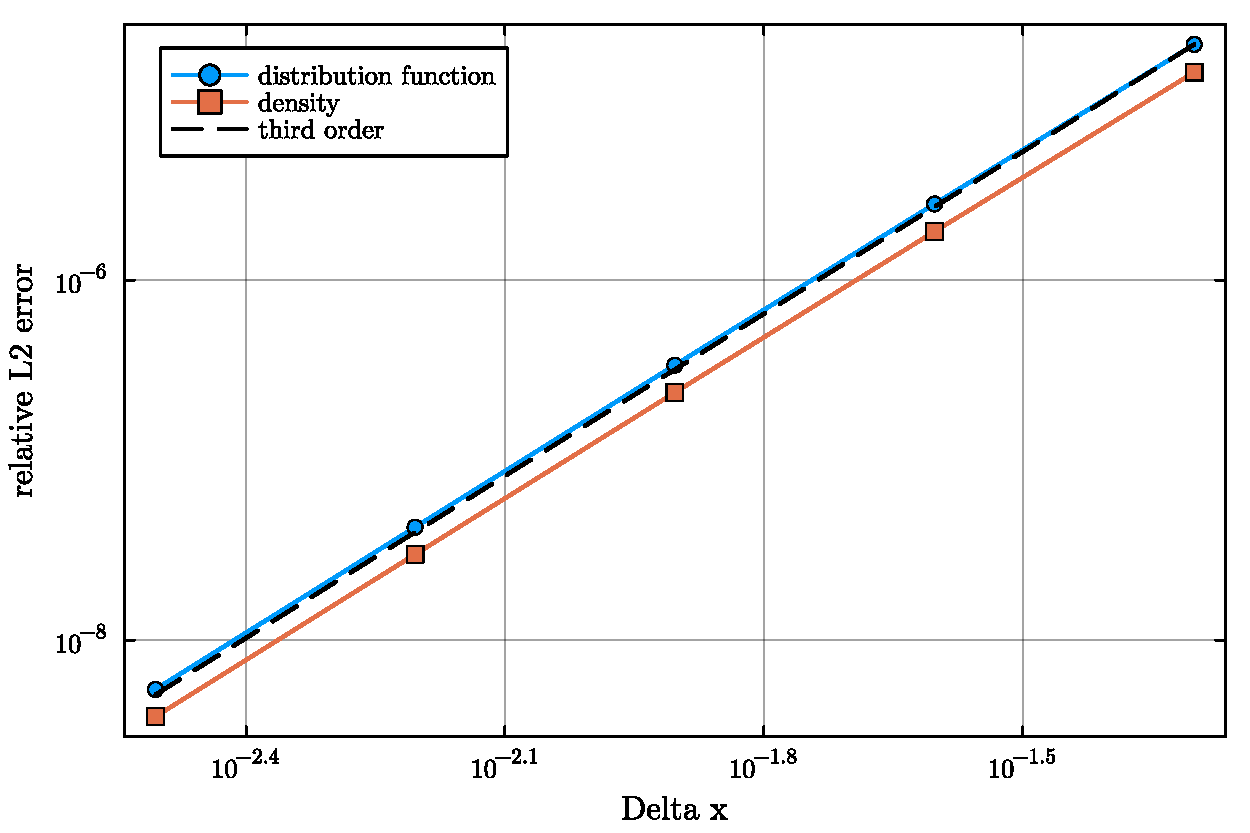
\includegraphics[width=0.62\textwidth]{figures/transport-convergence.pdf}
  \caption{Relative $L^2$ errors of the distribution function and density in the exact free-transport test.}
  \label{fig:transport-convergence}
\end{figure}

\subsection{Temporally over-resolved BGK test}

The full method combines third-order active flux transport with second-order Strang splitting. With a fixed molecular $\cfl$, $\Delta t=O(\Delta x)$ and the $O(\Delta t^2)$ splitting error masks third-order spatial convergence. To expose the spatial behavior while retaining Strang splitting, the time step is refined as
\begin{equation}
  \Delta t = C\frac{\Delta x^{3/2}}{v_{\max}},
  \label{eq:overresolved-step}
\end{equation}
so the global splitting error scales as $O(\Delta x^3)$. A uniform step is chosen to divide the final time exactly, avoiding a mesh-dependent shortened last step.

The periodic wave in Eq.~\eqref{eq:wave-initial} is evolved with $\mathrm{Kn}=10^{-2}$, $N_v=24$, and $t=0.005$. Since no closed-form BGK solution is available, an $N_x=640$ solution is restricted conservatively onto every comparison grid. Table~\ref{tab:bgk-convergence} and Fig.~\ref{fig:bgk-convergence} present the errors. The density error is smaller than the distribution error and enters its asymptotic range later. On the finest refinement, the distribution and density orders are $3.076$ and $3.002$, showing compatible third-order behavior. The slight value above three for the distribution is attributable to the finite-grid reference and pre-asymptotic error cancellation.

\begin{table}[htbp]
  \centering
  \caption{Convergence of the temporally over-resolved active flux BGK scheme.}
  \label{tab:bgk-convergence}
  \begin{tabular}{rrrrr}
    \toprule
    $N_x$ & $\|e_f\|_2$ & order & $\|e_\rho\|_2$ & order \\
    \midrule
     20 & $1.0052\times10^{-6}$  & --    & $2.3335\times10^{-7}$  & -- \\
     40 & $1.5458\times10^{-7}$  & 2.701 & $4.8229\times10^{-8}$  & 2.274 \\
     80 & $2.3965\times10^{-8}$  & 2.689 & $8.6949\times10^{-9}$  & 2.472 \\
    160 & $3.2627\times10^{-9}$  & 2.877 & $1.3437\times10^{-9}$  & 2.694 \\
    320 & $3.8680\times10^{-10}$ & 3.076 & $1.6767\times10^{-10}$ & 3.002 \\
    \bottomrule
  \end{tabular}
\end{table}

\begin{figure}[htbp]
  \centering
  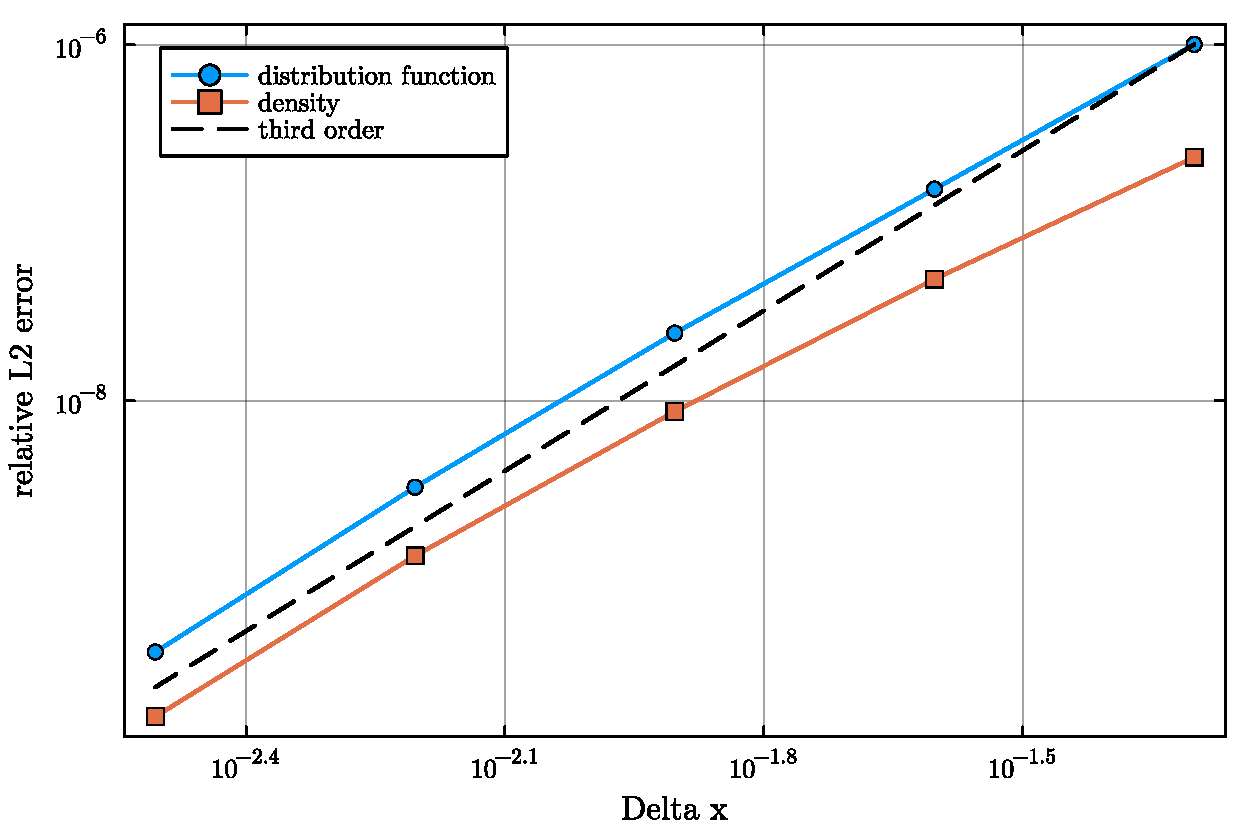
\includegraphics[width=0.62\textwidth]{figures/bgk-convergence.pdf}
  \caption{Relative $L^2$ errors of the distribution function and density in the temporally over-resolved BGK test. The reference solution uses $N_x=640$.}
  \label{fig:bgk-convergence}
\end{figure}

For a representative periodic computation with $N_x=200$, $N_v=48$, $\mathrm{Kn}=10^{-2}$, and $t=0.1$, the relative drift of mass, momentum, and energy is approximately $5.3\times10^{-14}$. Figure~\ref{fig:periodic-wave} shows the corresponding macroscopic profiles. These results confirm that the velocity-moment correction and conservative interface flux are consistent at the fully discrete level.

\begin{figure}[htbp]
  \centering
  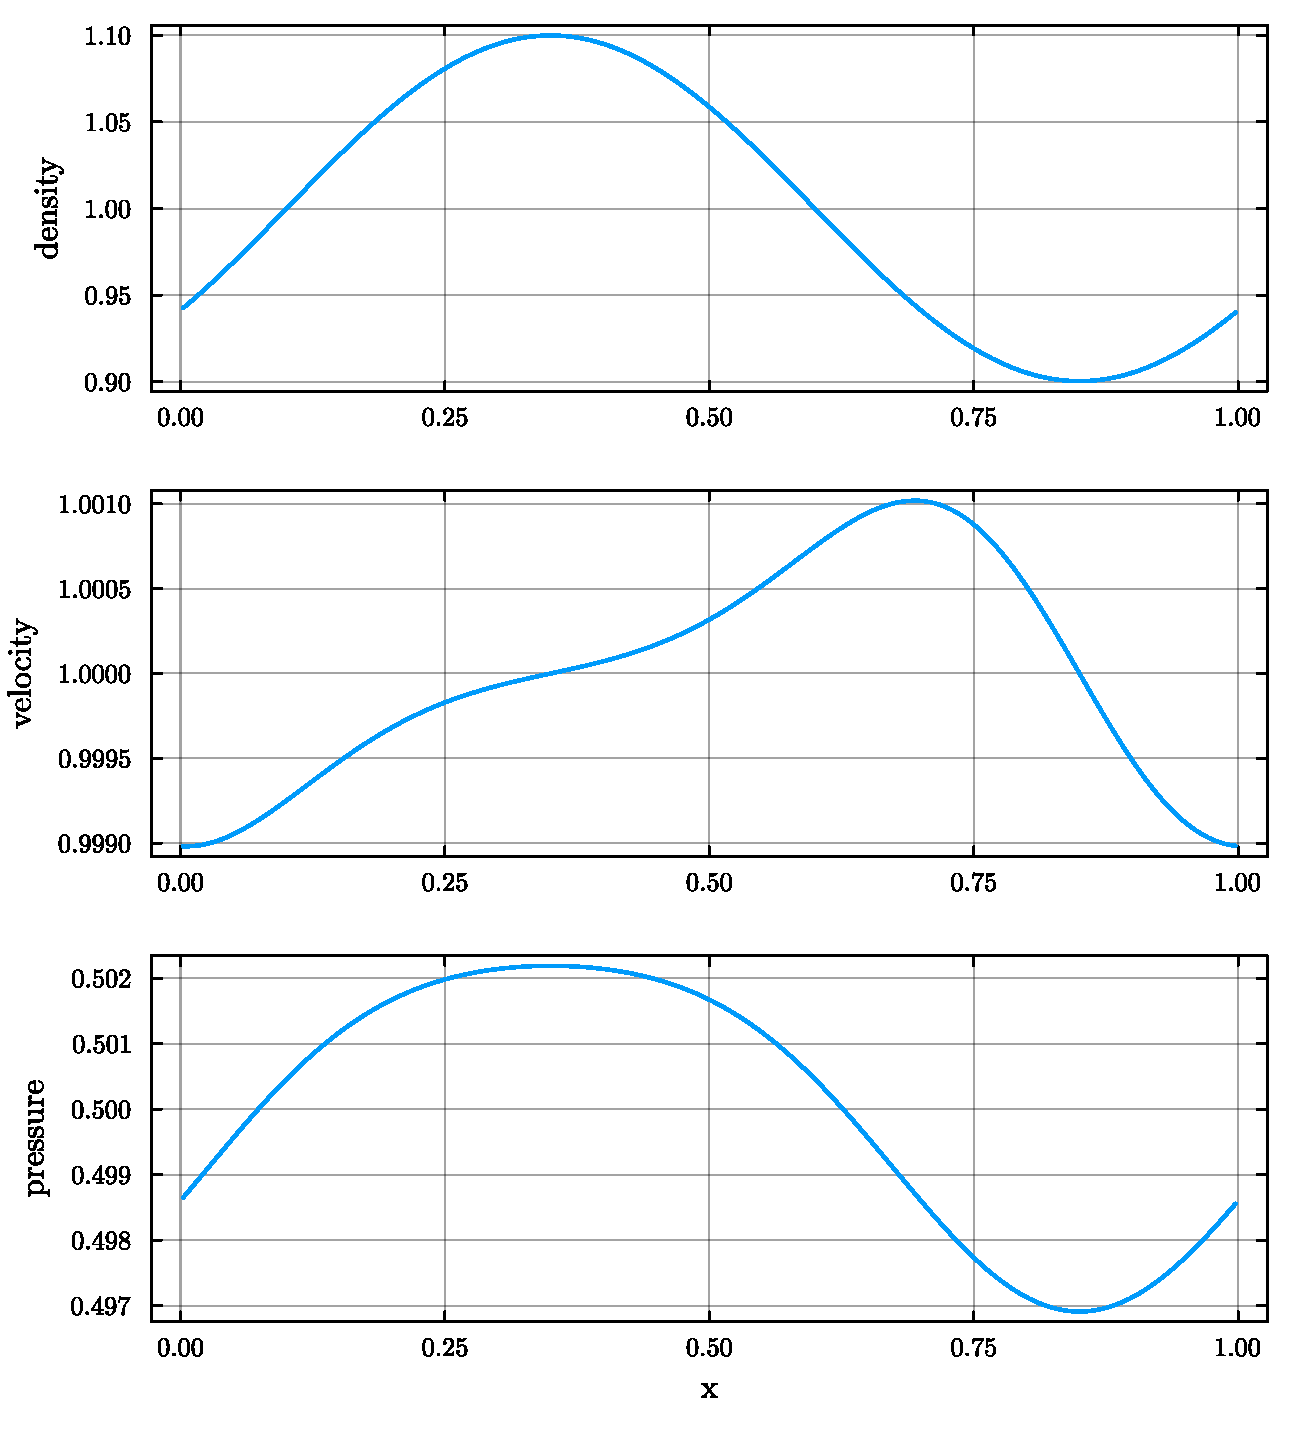
\includegraphics[width=0.64\textwidth]{figures/periodic-wave.pdf}
  \caption{Density, velocity, and pressure of the periodic BGK wave at $t=0.1$ with $N_x=200$, $N_v=48$, and $\mathrm{Kn}=10^{-2}$.}
  \label{fig:periodic-wave}
\end{figure}

\section{Sod shock tube}
\label{sec:sod}

The Sod problem \cite{sod1978survey} is employed to assess the shock-capturing and positivity properties. The initial states are
\begin{equation}
  (\rho,U,p)_L=(1,0,1),
  \qquad
  (\rho,U,p)_R=(0.125,0,0.1),
  \label{eq:sod-states}
\end{equation}
separated at $x=0.5$. Table~\ref{tab:sod-setup} lists the computational setup. The small Knudsen number places the BGK solution close to the inviscid Euler limit. At the initial discontinuity, right-moving particles take the left Maxwellian and left-moving particles take the right Maxwellian, which provides a kinetic upwind trace for the shared point value.

\begin{table}[htbp]
  \centering
  \caption{Computational setup of the Sod shock tube.}
  \label{tab:sod-setup}
  \begin{tabular}{ll}
    \toprule
    Quantity & Value \\
    \midrule
    Physical domain & $x\in[0,1]$ \\
    Physical cells & $N_x=200$ \\
    Velocity domain & $v\in[-5,5]$ \\
    Velocity points & $N_v=72$ \\
    Gas model & $K=0$, $\gamma=3$ \\
    Knudsen number & $10^{-4}$ \\
    Molecular CFL number & $0.45$ \\
    Final time & $0.12$ \\
    Boundary condition & fixed incoming Maxwellian reservoirs \\
    \bottomrule
  \end{tabular}
\end{table}

Figure~\ref{fig:sod} shows the density, velocity, and pressure, together with the exact Euler Riemann solution for $\gamma=3$. The rarefaction fan, contact wave, and right-moving shock propagate at the expected speeds. Density across the contact is more diffuse than the pressure and velocity because the kinetic jump sensor activates the upwind component over that region. Small smooth overshoots remain in the velocity plateau, but no negative cell-average distribution is produced. The simulation reaches $t=0.12$ in 263 steps, and the minimum cell-average distribution is $6.9\times10^{-17}$. The result demonstrates that the active flux representation can be extended from smooth kinetic transport to a discontinuous collisional flow when shock sensing and positivity control are included.

\begin{figure}[htbp]
  \centering
  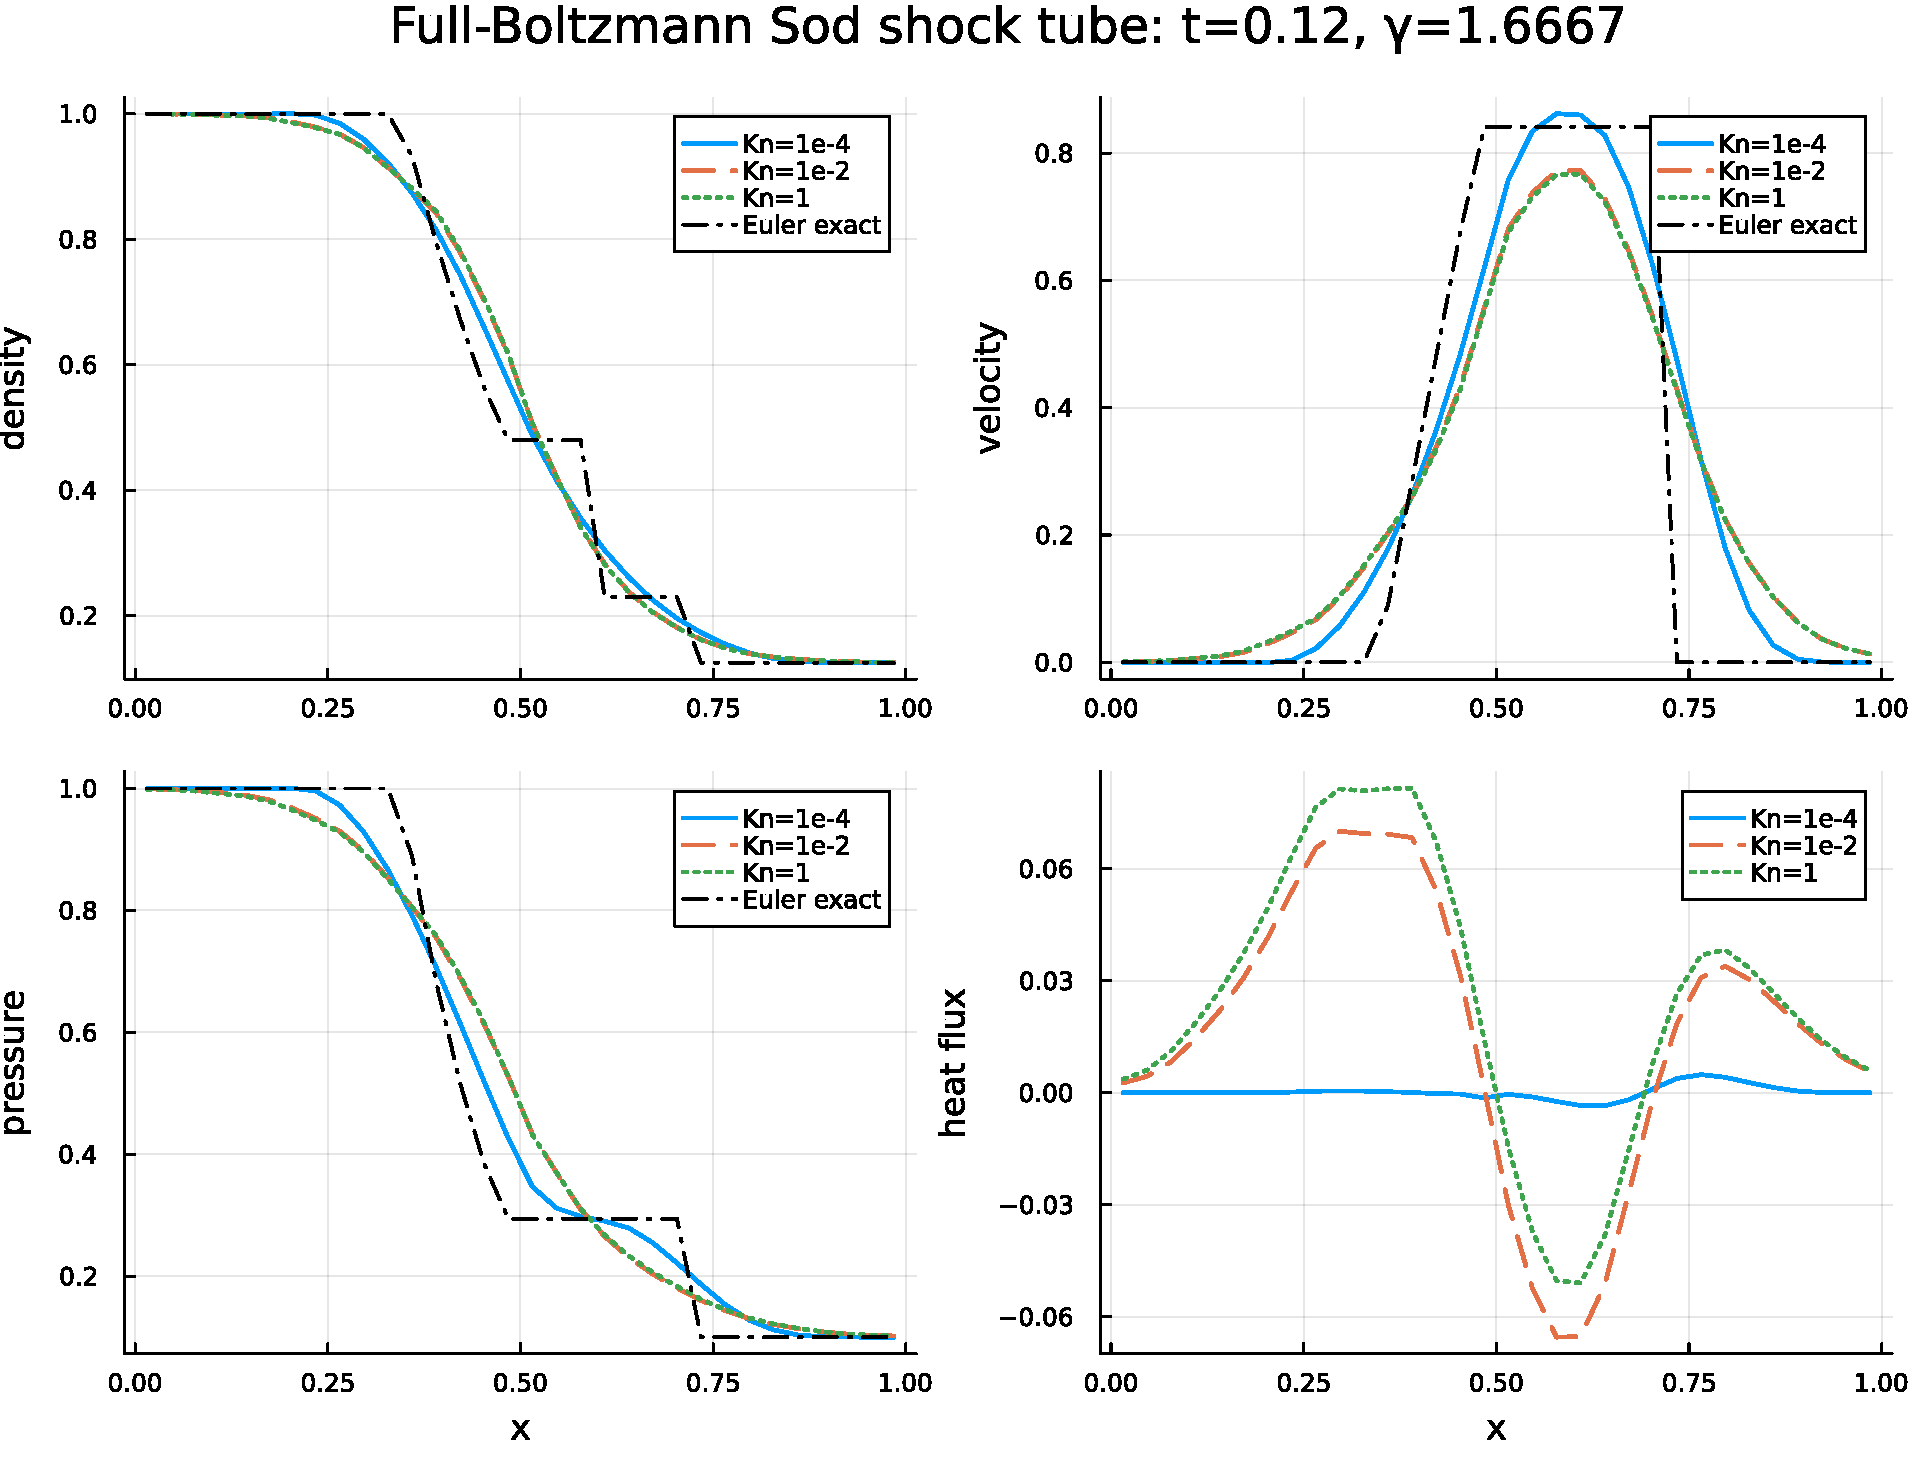
\includegraphics[width=0.82\textwidth]{figures/sod-shock-tube.pdf}
  \caption{Sod shock tube at $t=0.12$. The active flux BGK solution is compared with the exact Euler Riemann solution for $\gamma=3$.}
  \label{fig:sod}
\end{figure}

\section{Conclusion}
\label{sec:conclusion}

Kinetic equations provide a direct connection between particle transport and macroscopic flow evolution, but their phase-space dimensionality places strong demands on numerical resolution. In this paper, an active flux kinetic scheme has been formulated for the one-dimensional BGK equation. Cell averages and shared interface values define a compact continuous reconstruction, while molecular characteristics evolve the point values and provide conservative time-averaged fluxes. Pointwise Gaussian relaxation preserves the spatial accuracy of the nonlinear source, and the corrected discrete Maxwellian conserves the quadrature moments to roundoff. The exact transport experiment identifies third-order convergence of both the distribution and density. With temporal over-resolution, the complete BGK algorithm reaches the same spatial rate despite the second-order Strang splitting. The shock-limited formulation remains positive and captures the principal structures of the Sod problem.

The current method provides a compact framework for further development of collisional active flux solvers. The next step is to replace the BGK relaxation by the full Boltzmann collision operator, for example through a fast spectral formulation, while retaining the active flux transport and discrete conservation treatment. Multi-dimensional physical and velocity spaces, less dissipative bound-preserving limiters, gas-surface interaction, and asymptotic-preserving time integration are also natural extensions. These developments may lead to an efficient high-order tool for cross-scale and non-equilibrium flow simulation.

\section*{CRediT authorship contribution statement}

\textbf{Tianbai Xiao:} Conceptualization, Methodology, Software, Formal analysis, Investigation, Visualization, Writing -- original draft, Writing -- review \& editing.

\section*{Declaration of competing interest}

The author declares that there are no known competing financial interests or personal relationships that could have appeared to influence the work reported in this paper.

\section*{Data and code availability}

The Julia programs used to produce the numerical results are included in the \texttt{src/} directory of the accompanying repository. The LaTeX manuscript and generated figures are provided in \texttt{tex/}. No external experimental data are required.

\bibliographystyle{elsarticle-num}
\bibliography{references}

\end{document}
